\documentclass[11pt]{article}
\usepackage[margin=1in]{geometry}          
\usepackage{graphicx}
\usepackage{amsthm, amsmath, amssymb}
\usepackage{setspace}\onehalfspacing
\usepackage[loose,nice]{units}
\usepackage{array}
\usepackage[super]{nth}
\usepackage{graphicx}
\usepackage{float}
\usepackage{algpseudocode}
\usepackage[linesnumbered,ruled,vlined]{algorithm2e}
\usepackage{subcaption}
\usepackage{mathtools}
\usepackage[displaymath, mathlines]{lineno}
\usepackage{natbib}
\usepackage[all]{nowidow}
\newenvironment{conditions}
  {\par\vspace{\abovedisplayskip}\noindent\begin{tabular}{>{$}l<{$} @{${}={}$} l}}
  {\end{tabular}\par\vspace{\belowdisplayskip}}
% nicer math
\let\vec\mathbf
\newcommand{\R}{\mathbb{R}}  
\newenvironment{process}[1][htb]
  {\renewcommand{\algorithmcfname}{Process}% Update algorithm name
   \begin{algorithm}[#1]%
  }{\end{algorithm}}

\title{Role-Model Choice Probability Regression}
\author{Saar Egozi and Yoav Ram}
\date{13/05/2020}

\begin{document}

\begin{titlepage}
\maketitle
\end{titlepage}

\section*{Role-Model Choice Process}
Consider a population of~$N$ role-models and copiers.
Copiers choose their role-models one by one.
We denote the number of copiers that chose role-model~$j$ after $i$~copiers have made their choice by $K_{i,j}$, such that $\sum_{j=1}^N{K_{i,j}} = i$. 
The stochastic process of role-model choice, 
\begin{equation} \label{eq:process}
\big\{\vec{K}_i\big\}_{I=1}^N, \quad \vec{K}_i=(K_{i,1}, \ldots, K_{i,N}),
\end{equation}
is described by the recurrence equation
\begin{equation} \label{eq:recurrence}
K_{i,j} = K_{i-1,j} + S_{i,j}, \quad i,j=1,2,\ldots,N
\end{equation}
where $S_{i,j}=1$ if the $i$-th copier chose role-model~$j$ and 0 otherwise, and the initial state is $K_{0,j}=0$.

The probability $P_{i,j}=P(S_{i,j}=1)$ that the $i$-th copier chose role-model $j$ is called the \emph{prestige} of role-model~$j$ in the eyes of copier~$i$.
This prestige $P_{i,j}$ is determined as follows.
First, role-model~$j$ is characterized by its indicator values $A_j$.
Copier~$i$ estimates the indicator value of role-model~$j$, such that the estimated indicator value is
\begin{equation}
A_{i,j} = A_j + e_i,
\end{equation}
where $e_i$ is the estimation error of copier $i$. 
Then, a bias function is applied to the estimated indicator value,
\begin{equation}
\beta(A_{i,j}) = b \cdot \exp{\Big(-\frac{(A_{i,j} - \hat{A})^2}{2J}\Big)},
\end{equation}
where $\hat{A}$ is the optimal indicator value and $J$ is a bias coefficient.
Finally, the prestige $P_{i,j}$ of role-model~$j$ in the eyes of the $i$-th copier is determined by the estimated biased indicator value $\beta(A_{i,j})$ and the influence $K_{i-1,j}$, 
\begin{equation}
P_{i,j} = \frac{\alpha_j \cdot \beta(A_{i,j}) + (1-\alpha_j) \cdot K_{i-1,j}}{W_i},
\end{equation}
where the weight $\alpha_j$ is a characteristic of role-model~$j$ that determines the relative significance of the indicator and the influence in the prestige, and $W_i$ is a normalizing factor to ensure $\sum_{j=1}^N{P_{i,j}}=1$,
\begin{equation}
W_i = \sum_{j=1}^N{\Big(\alpha_j \cdot \beta(A_{i,j}) + (1-\alpha_j) \cdot K_{i-1,j}\Big)}.
\end{equation}

In the following, we will analyze the stochastic process $\{\vec{K}_{i}\}_{I=1}^N$ to show the following results:
\begin{enumerate}
\item $\mathbb{E}[K_{N,j}] = N \cdot P_{1,j}$ if $e_i=e_k$ for all $i,k$. That is, the expected number of copiers of role-model~$j$ equals its prestige in the eyes of the first copier, multiplied by the total number of copiers. Moreover, we find that $\mathbb{E}[K_{N,j}] = \beta(A'_j) \; / \; \overline{ \beta(A') }$, where $A'_j$ is the estimated indicator value and $\overline{ \beta(A') }$ is the population mean estimated indicator value. That is, the expected number of copiers of a role-model equals its relative biased indicator value, similar to the role of relative fitness in population-genetic models.
\item The role-model choice process (eq.~\ref{eq:process}) is equivalent to a P\'{o}lya urn model if $e_i=e_k$ for all $i,k$. Therefore, $\vec{K}_i = (K_{i,1}, \ldots, K_{i,N})$ follows a Dirichlet-Multinomial distribution,
\begin{equation}
\vec{K}_i \sim \mathit{DM}\big(i, \vec{P}_1\big), %TODO check I didn't mess up the parameterization of DM
\end{equation}
where $\vec{P}_1 = (P_{1,1}, \ldots, P_{1,N})$.
Note that here $P_{i,j}$ is only a function of the indicator values $A_j$ and the weights $\alpha_j$.
\end{enumerate}


\pagebreak

Consider a population that consists of $N$ role-models and $N$ copiers.
Each copier chooses a role-model as described in the process below, based on several factors:
Let $A_j$ be the indicator value of role-model $j$; $e_i$ is the estimation error of the indicator value of copier $i$;
$K_{i,j}$ is the number of copiers that chose role-model $j$, after the $i$-th copier chose a role-model;
$\beta(A_{i,j})$ is the bias function applied to an estimated indicator value $A_{i,j} = A_j + e_i$;
$\alpha_j$ is the indicator weight in the prestige score of role-model $j$, $\alpha_j \in [0,1]$ for all $j \in N$;
$G_{i,j}$ is the prestige score role-model $j$ has when the $i$-th copier is about to choose a role-model;
$\widetilde{G_{i,j}}$ is the normalised prestige score, which is the probability that the $i$-th copier will choose role-model $j$.
The stochastic process of calculating how many copiers each role-model will have after all $N$ copiers chose a role-model (i.e $K_N$) is described below:

\begin{process}\caption{Sequential stochastic choosing process}
\label{stochastic_process}
\setstretch{1.35}
\DontPrintSemicolon
\KwIn{$N,\eta,\alpha,\hat{A},b,J$}
\KwOut{K}
$K_{0,j} \gets 0$  for all $j \in N$\;
\For{$i \gets 1$ \KwTo $N$}{
\For{$j \gets 1$ \KwTo $N$}{
$A_{i,j} \gets A_j + e_i$\;
$\beta(A_{i,j}) \gets b \cdot e^{-\frac{(\hat{A} - A_{i,j})^2}{2J}}$\;
$G_{i,j} \gets \alpha_i\cdot\beta(A_{i,j}) + (1-\alpha_i)\cdot K_{i-1,j}$ \label{prestige_eq}\;
}
\For{$j \gets 1$ \KwTo $N$}{
$\widetilde{G_{i,j}} \gets \frac{G_{i,j}}{\sum\limits_{m=1}^{N} G_{i,m}}$\label{prob_prestige}\;
}
Draw $j'$ from a categorical distribution with probability vector $\widetilde{G_i}$ such that the probability to draw $j$ is $\widetilde{G_{i,j}}$ \label{draw_role_model}\;
\For{$j \gets 1$ \KwTo $N$}{
\eIf{$j'==j$}{
$S_{i,j}\gets1$\;
} {
$S_{i,j}\gets0$\;
}
$K_{i,j} \gets K_{i-,j} + S_{i,j}$\;

}
}
\end{process}

Process \ref{stochastic_process} is sequential in nature, where each step depends on the one before it, line \ref{prestige_eq} (i.e $G_{i,j}$ depends on the value of the $i-1$ choice).
We therefore look for a function that estimates the results beforehand, since we can't use parallel computations when simulating such a process, and it is also hard to analyse mathematically.

\section*{General Binomial Distribution approximation}
Process \ref{stochastic_process} resembles a binomial distribution, with some exceptions, when observing the number of copiers a specific role-model will have.
We'll use the generalised binomial distribution defined by \citet{GBD} to find a function that will estimate the number of copiers role-model $j$ will have, based solely on $A_j$, rather than taking into consideration the number of copiers during the choosing process.
\paragraph{Lemma: } $E[K_{N,j}] = N \cdot \widetilde{G_{1,j}}$, when $e_i=e_j$ for all $i,j \in N$, where $K_{N,j}$ is the number of copiers of role-model $j$ after all $N$ choices were made,
 and $\widetilde{G_{1,j}}$ is the probability that the first copier will choose role-model $j$.
\paragraph{Proof: } We'll denote $Q_j(k,i)$ as the probability that exactly $k$ out of $i$ copiers will choose role-model $j$, using conditional probability:
\begin{equation}\label{recursive}
Q_j(k,i) = P_j(S_{i,j}=1 | k-1,i-1) \cdot Q_j(k-1,i-1) + P_j(S_{i,j} =0 | k,i-1) \cdot Q_j(k,i-1)
\end{equation}
where $S_{i,j} =1 $ when the $i$-th copier chooses role-model $j$.

Equation \ref{recursive} is equivalent to equation (2.1) that \citet{GBD} define.
$Q_j(k,N)$ is the probability that $k$ out of $N$ copiers choose role-model $j$ at the end of the process, which by our previous notation is $K_{N,j}$.
In \citep[Eq. 2.3]{GBD}, they show that the expected value of $k$ is: $E[k] = N \cdot Q_j(1,1)$ (using different notations).
$Q_j(1,1)$ is the initial probability to choose role-model $j$, before any choices are made.
$Q_j(1,1) = \widetilde{G_{1,j}}$ by definition, therefore we can say that $E[K_{Nj}]=N \cdot\widetilde{G_{1,j}}$.\\

\paragraph{Analysis: } 
For simplicity we'll assume $\alpha = \alpha_i=\alpha_j$ for all $i,j \in N$, and compute $\widetilde{G_{1,j}}$:
\begin{equation}\label{initial_prob}
\widetilde{G_{1,j}} = \frac{\alpha\beta(A'_j)}{\sum\limits_{k=1}^{N}\alpha\beta(A'_k)}
\end{equation}
where $A'_j = A_j + e$, $e=e_i$ for any $i \in N$.
The denominator of equation \ref{initial_prob} can also be formulated as:
\begin{equation}
 \sum\limits_{k=1}^{N}\alpha\beta(A'_k) = \alpha N \cdot \overline{\beta(A')}
\end{equation}
where $\overline{\beta(A')}$ is the mean value of $\beta(A'_k)$ for all $k$.
We now can write $E[K_{Nj}]$ as:
\begin{equation}
E[K_{Nj}] = \frac{\beta(A'_j)}{\overline{\beta(A')}}
\end{equation}
where the only variable is $A'_j$, because $\overline{\beta(A')}$ is the mean of the distribution we draw the indicator values from, modified by some constant parameters in $\beta$.
We can then denote $\frac{1}{L} = \overline{\beta(A')}$ and write:

\begin{equation}\label{linearEq}
E[K_{Nj}] = L\cdot \beta(A'_j)
\end{equation}

\paragraph{Result: } The expected number of copiers of role-model $j$ at the end of the stochastic process is: $E[K_{Nj}] = L\cdot \beta(A'_j)$ for some constant L (i.e linear relation) when $\alpha$ is homogenous and estimation errors $e$ are homogenous.

\begin{figure}
    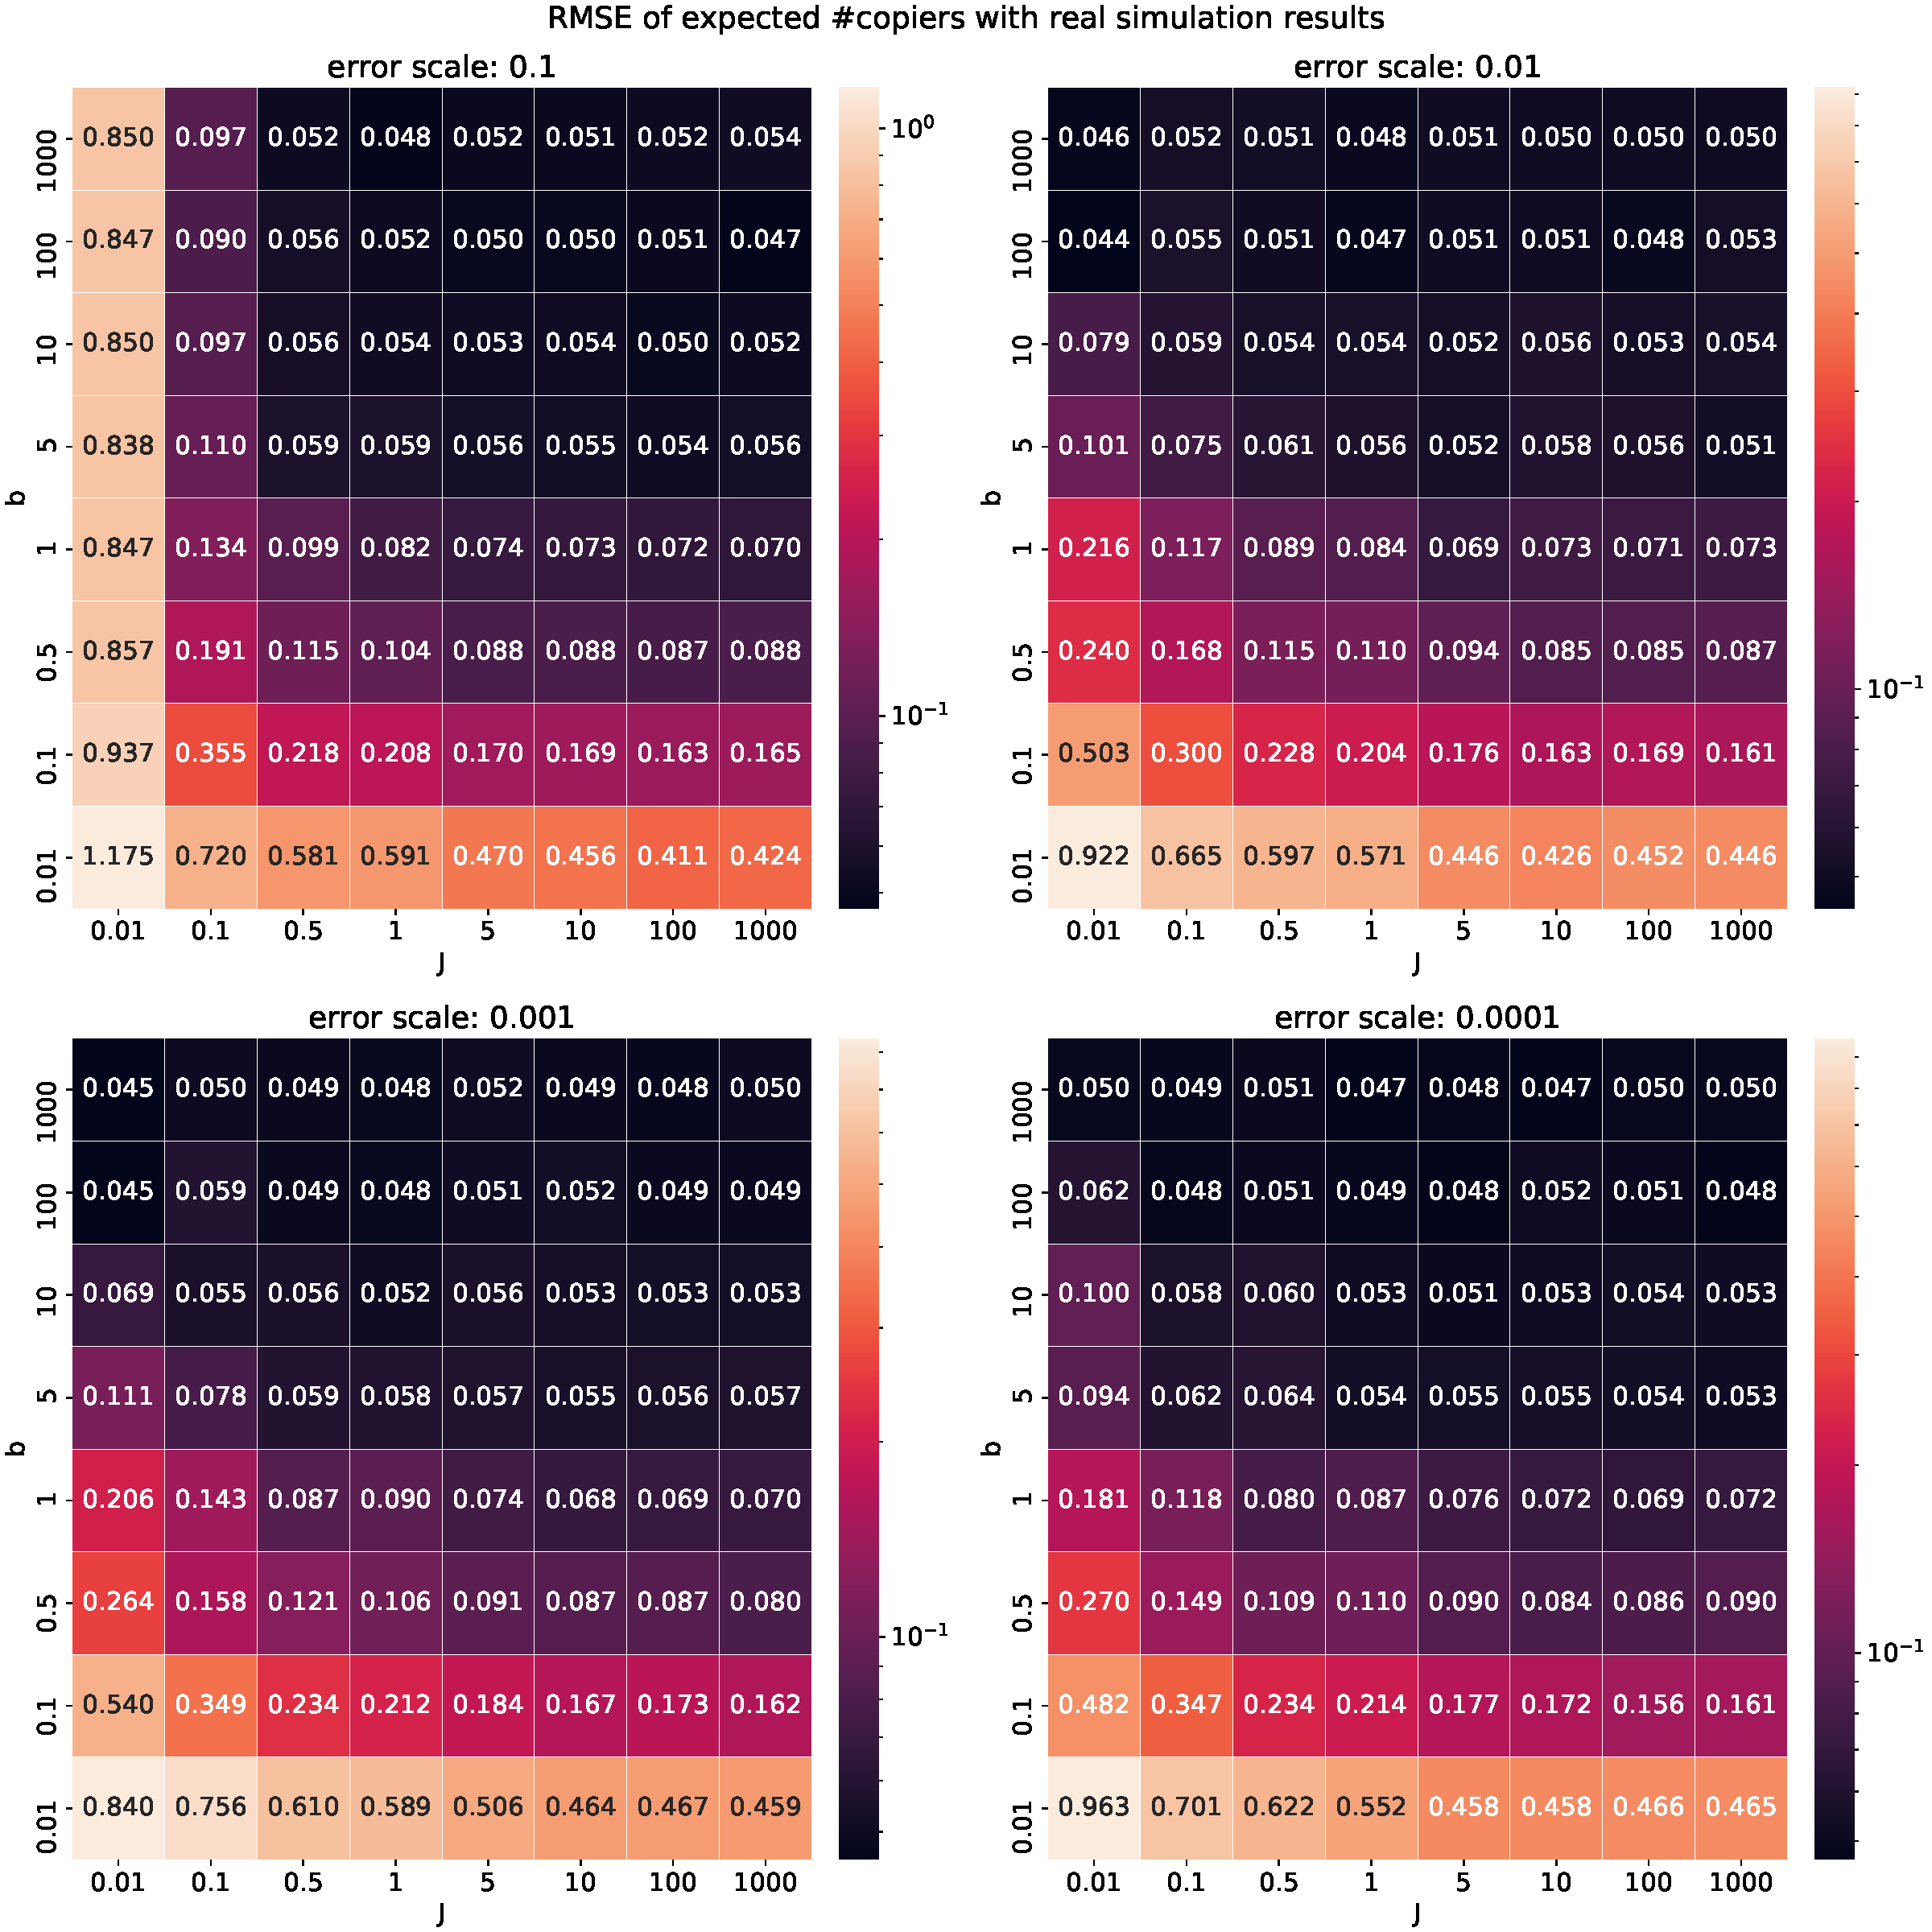
\includegraphics[width=\linewidth]{GBD_rmse_heatmap.pdf}
    \caption{RMSE graphs between the model results and the expected values based on Eq. \ref{linearEq}, for a population of $N=400$}
    \label{RMSE}
\end{figure}

\begin{figure}
    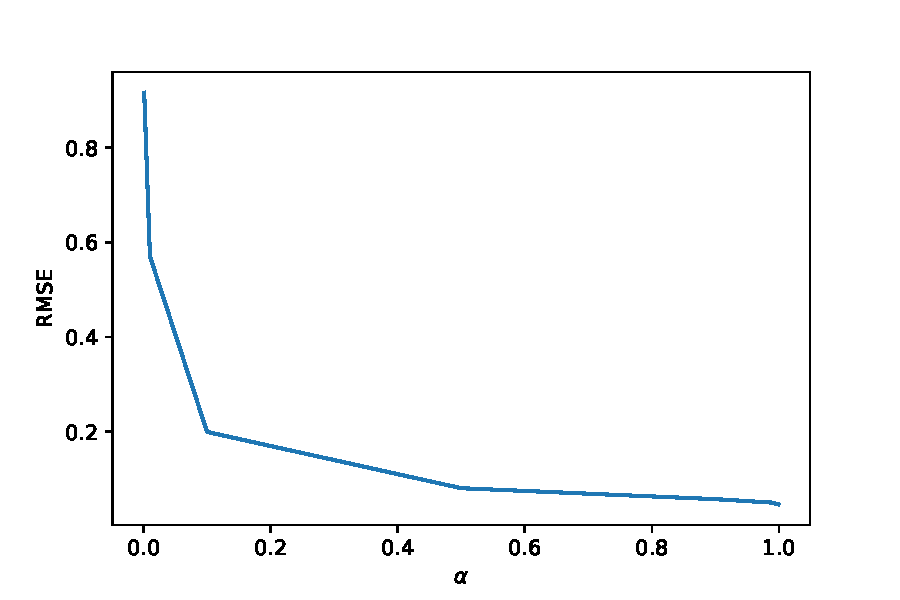
\includegraphics[width=\linewidth]{alpha_rmse.pdf}
    \caption{RMSE between the model results where $b=1,j=1,\eta=0.01$ and the expected values based on Eq. \ref{linearEq}, for a population of $N=400$}
    \label{RMSE:alpha}
\end{figure}

\paragraph{Numeric results:} To test our approximation for heterogenous estimation errors ($e_i \ne e_j$), we simulated the stochastic process described above 400 times over a population of 400 individuals.
We calculated the Root Mean Square Error (RMSE) between the average of the model's results and the expected values using Eq. \ref{linearEq}.
 We simulated the process for several values of: $b,J,\eta,\alpha$ ($e_i \sim N(0,\eta^2)$).
 In figure \ref{RMSE} we see that the RMSE is $\le 0.2$ in more than 70\% of the cases, and not more than 1.2 for any set of parameters.
 We can also see in figure \ref{RMSE:alpha} that for very small values of $\alpha$, the RMSE is still lower than 1. 
We consider these values acceptable because a deviation of 1 copier more or less for a large number of iterations is insignificant. 
We expect that the larger the population, and the larger the number of simulations, our approximation become more precise.

\clearpage

\section*{Dirichlet-Multinomial distribution approximation}
\paragraph{Reminder: \textit{Pólya urn model}}  is a stochastic process that is defined as such: 
The process consists of $N$ draws from an urn with an initial amount of coloured balls. When a ball is drawn, it is then placed back in the urn together with an additional new ball of the same colour.\\
Let $\overrightarrow{U_i} = \{u_{i,1},u_{i,2},...,u_{i,M}\}$  where $u_{i,j}$ is the number of balls of the $j$-th colour in the urn after $i$ draws.
Let $S_{i,j}=1$ when drawing a $j$ coloured ball on the $i$-th draw, and $0$ otherwise. The probability that $S_{i,j}=1$ is:
\begin{equation}\label{polya}
\begin{split}
P(S_{i,j} = 1 | \overrightarrow{U_{i-1}}) & = \frac{u_{i-1,j}}{\sum\limits_{m=1}^{M} u_{i-1,m}}\\\\
 & = \frac{o_j + w_{i-1,j}}{\sum\limits_{m=1}^{M} o_m + w_{i-1,m}}\\\\
 & = \frac{o_j + w_{i-1,j}}{i-1 + \sum\limits_{m=1}^{M} o_m}
\end{split}
\end{equation}
where $o_j$ is the initial number of balls of the colour $j$ in the urn, and $w_{i,j}$ is the number of new balls that were added to the urn after $i$ draws of the colour $j$.

\paragraph{Proposition:} Process \ref{stochastic_process} is equivalent to a \textit{Pólya urn model} when $e=e_i=e_j$ and $\alpha=\alpha_j=\alpha_i$ for all $i,j \in N$.
\paragraph{Proof:} 
Using line \ref{prestige_eq} of Process \ref{stochastic_process} and a new notation $G'_{i,j} = \frac{G_{i,j}}{1-\alpha}$ we get:
\begin{equation}\label{odd_prestige}
\begin{split}
G'_{i,j} & = \frac{\alpha}{1-\alpha}\cdot \beta(A'_j) + \frac{1-\alpha}{1-\alpha}\cdot K_{i-1,j}\\\\
& = \alpha'\beta(A'_j) + K_{i-1,j}
\end{split}
\end{equation}
where $\alpha'$ is the odd ratio between the weight of the biased indicator value $\beta(A'_j)$ and the influence $K_{i,j}$.
Using line \ref{prob_prestige} of Process \ref{stochastic_process} and equation \ref{odd_prestige}, we calculate the probability that the $i$-th copier will choose role-model $j$:
\begin{equation}\label{copier_choose}
\begin{split}
\widetilde{G_{i,j}} = \frac{G_{i,j}}{\sum\limits_{m=1}^{N} G_{i,m}} &= \frac{G'_{i,j}}{\sum\limits_{m=1}^{N} G'_{i,m}}\\\\
&= \frac{\alpha'\beta(A'_j) + K_{i-1,j}}{\sum\limits_{m=1}^{N} \alpha'\beta(A'_m) + K_{i-1,m}}\\\\
& =\frac{\alpha'\beta(A'_j) + K_{i-1,j}}{i-1 + \sum\limits_{m=1}^{N} \alpha'\beta(A'_m)}
\end{split}
\end{equation}
Equations \ref{polya} and \ref{copier_choose} are equivalent when setting $M=N$, $o_j = \alpha'\beta(A'_j)$, $w_{i,j} = K_{i,j}$, therefore Process \ref{stochastic_process} is identical to a \textit{Pólya urn model}.

\paragraph{Application:}
In their paper, \citet[section 2]{dirichlet} prove that the proportion of different coloured balls in a \textit{Pólya urn model} will converge to the Dirichlet distribution as the number of draws approaches infinity, based on \textit{Martingale Convergence Theorem}.
We can therefore sample from a Dirichlet-Multinomial distribution to approximate how many copiers each of the role-models will have:
$\overrightarrow{K_i} \sim DirMul(N,\overrightarrow{G'_0})$.

\paragraph{Numeric results:}
Fig \ref{dirichlet_rmse} shows the root mean square errors between Process \ref{stochastic_process} and a stochastic process that determines the number of copiers based on draws from the Dirichlet-Multinomial distribution.
We see that the RMSE are mainly around 0.07, and not larger than 1.2, same as before.

\paragraph{Corollary:} We relax our assumption that $\alpha$ is homogenous, so $\alpha_j$ is the weight of the indicator value of role-model $j$.
$G_{i,j}$ is divided by its own $\alpha_j$, so $G'_{i,j}=\alpha'_i\beta(A'_j) + K_{i,j}$.
The proof remains the same, when using $\overrightarrow{G'_{0}}$ as the initial state. 
This means that we can assign each role-model with its own $\alpha_j$ value and still use the Dirichlet-based approximation.

\begin{figure}
    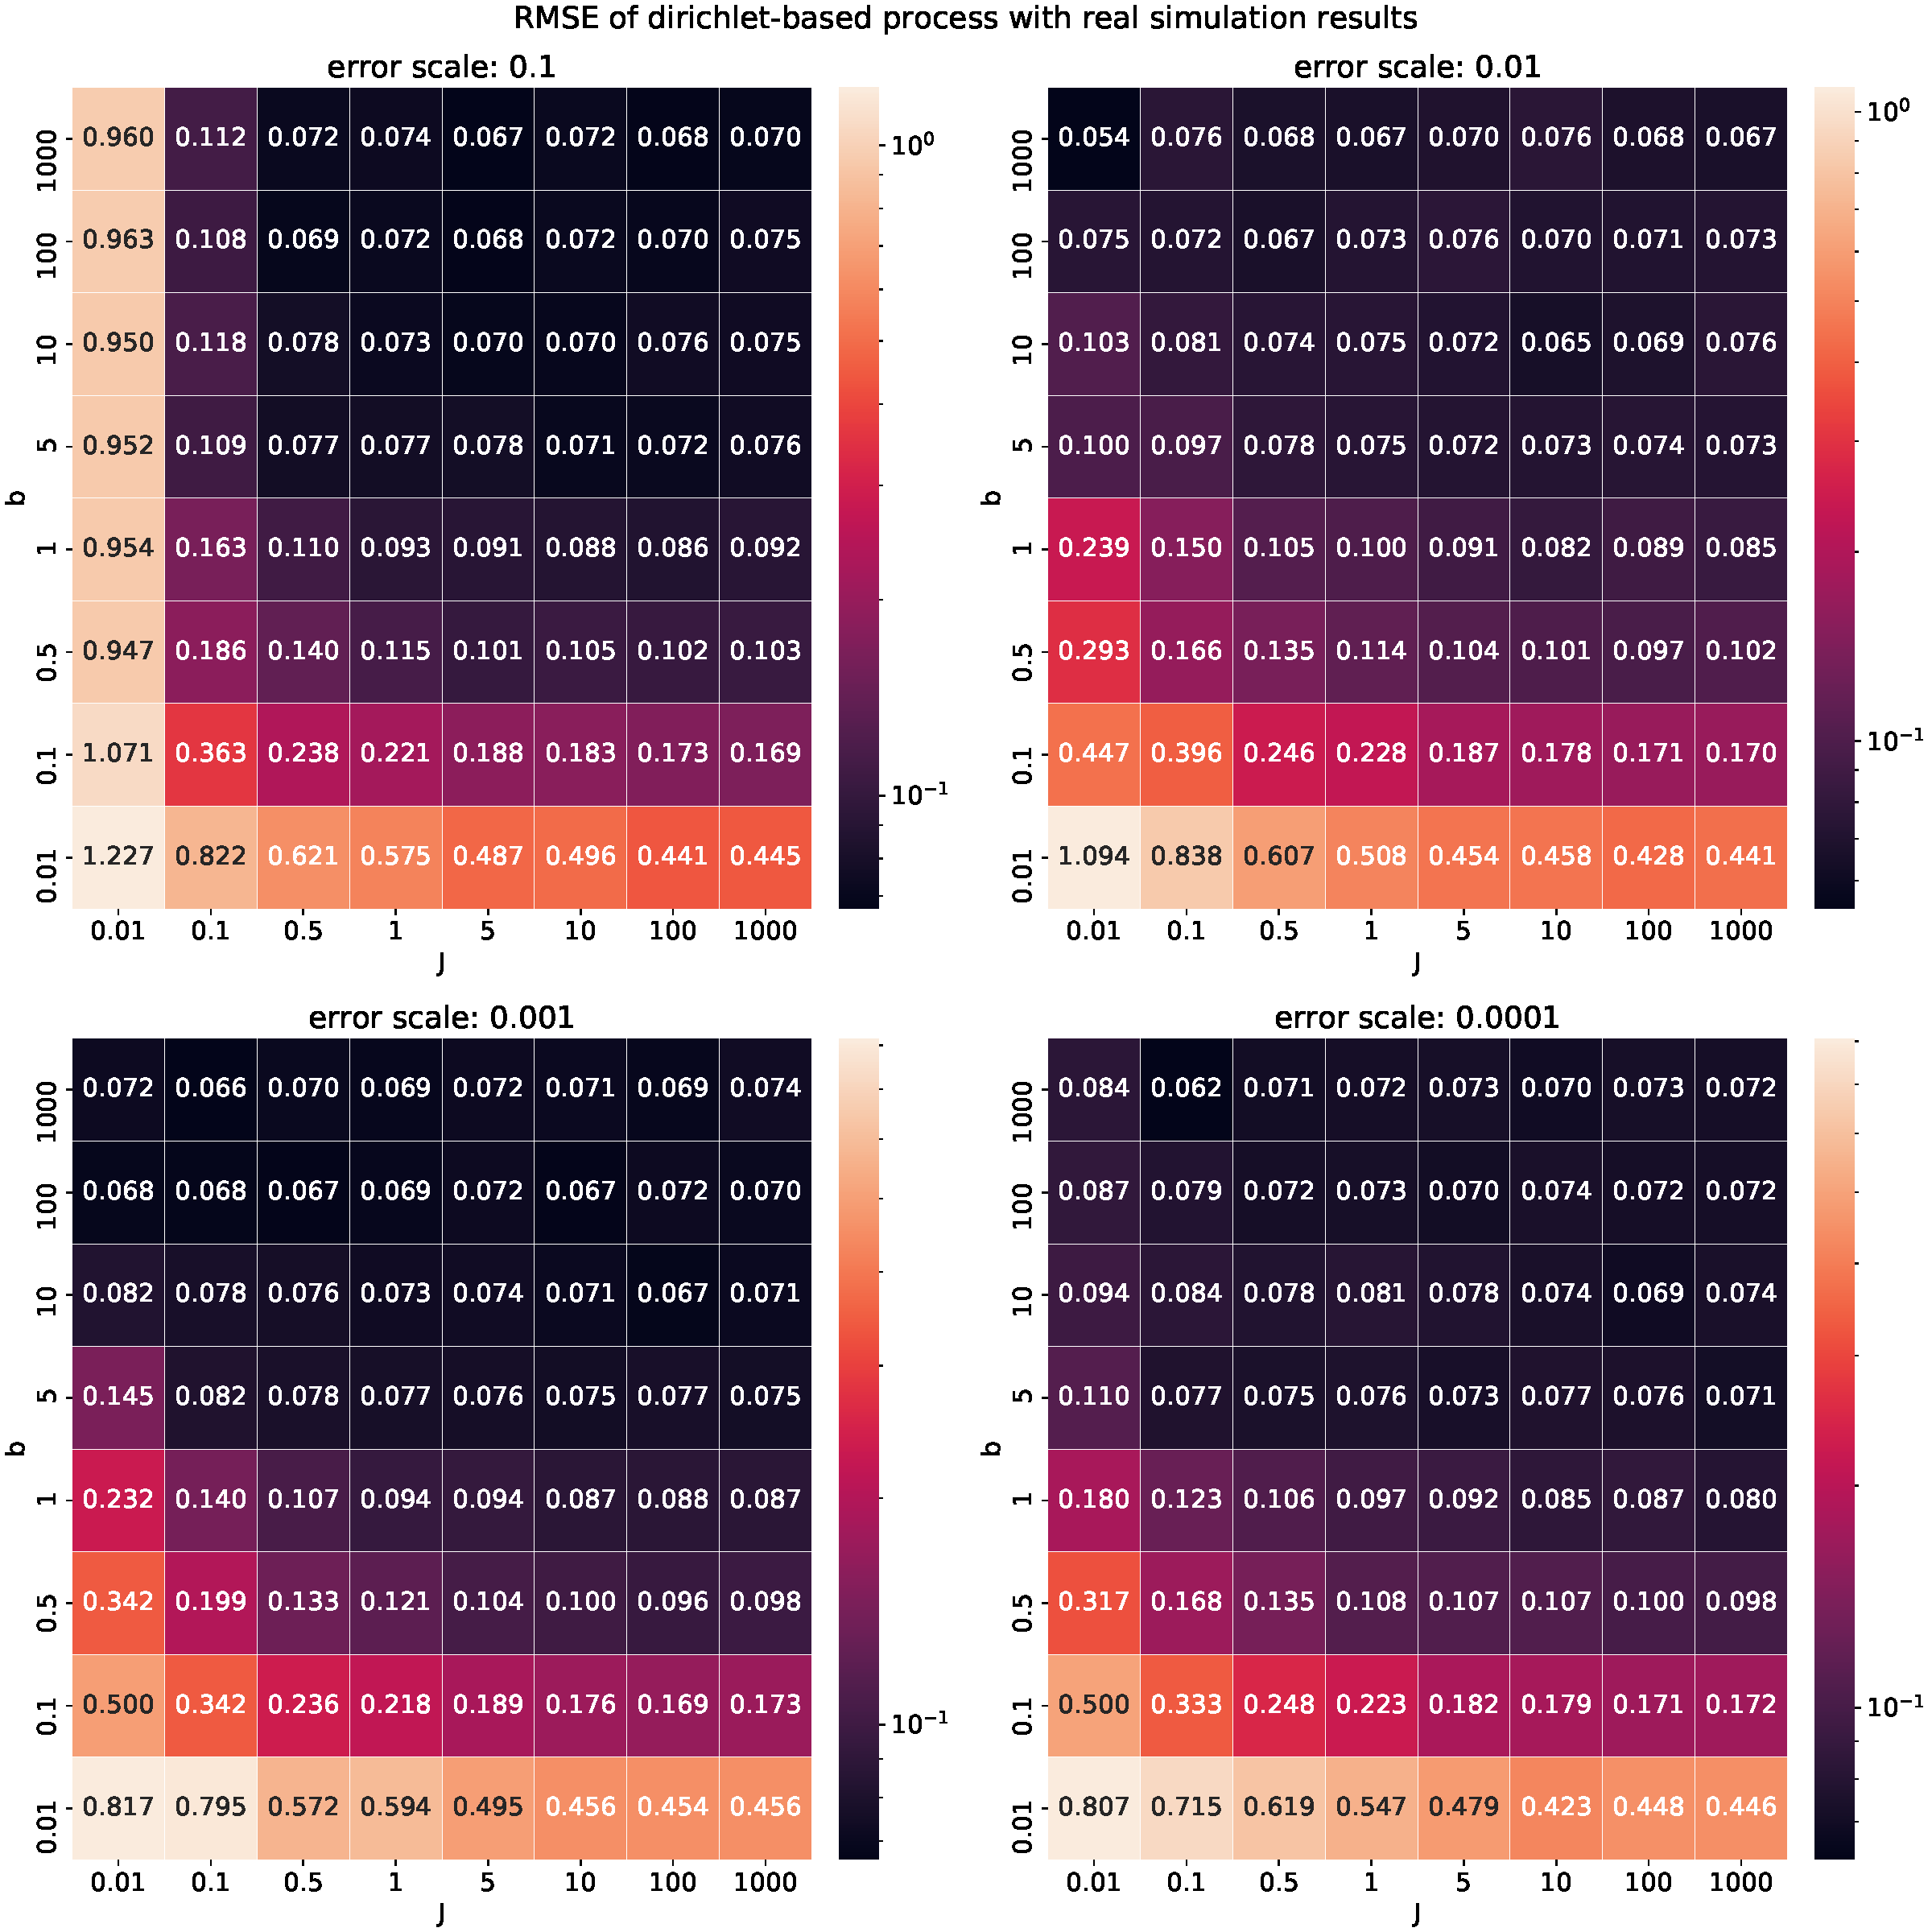
\includegraphics[width=\linewidth]{dirichlet_rmse_heatmap.pdf}
    \caption{RMSE graphs between the stochastic process by Algorithm 1 and a dirichlet-based process}
    \label{dirichlet_rmse}
\end{figure}



\clearpage
\bibliography{refs}
\bibliographystyle{apalike}
\end{document}